\documentclass[12pt]{myland}
\usepackage{pgfplots}

%%% Formatting
\def\<#1>{\texttt{#1}}
\setlength{\parskip}{1em}

%%%%%%%%%%%%%%%%%%%%%%%%%%%%FILE TITLE%%%%%%%%%%%%%%%%%%%%%%%%%%%%%%%%%%%%
\begin{document}

\title{CSE 444: \<SimpleDB> Final Report}
\author{Linxing Preston Jiang}
\maketitle

\section{Overall System Architecture}
	\label{overview}

	\par In a typical database architecture, there are four main components: Process Manager, Query Executor, Share
Utilities, and Storage Manger \cite{lecture3}. For our implementation of \<SimpleDB> in the labs,
the focus is on the Storage Manager and Query Executor: adding access methods for data stored on disk in lab1, adding both file
mutability (insert/delete tuples to/from file system, eviction from a full BufferPool) and query operators (SeqScan, Join,
etc.) \& aggregates (min, max, etc.) in lab2, adding the lock manager in lab3, adding the log manager in lab4, and finally, adding
parallel data processing ability in lab6 \cite{db}.

    Figure \ref{fig:architecture} shows the parts of the architecture of \<SimpleDB> which we implemented in the labs.
    \begin{figure}[h]
        \begin{mybox}
            \begin{tikzpicture}[
            >=latex,shorten >=2pt,shorten <=2pt,shape aspect=1,
        ]
            \tikzstyle{cyl} = [cylinder, shape border rotate=90, draw, minimum height=1cm, minimum width=5cm]
            \tikzstyle{noo} = [rectangle, draw, minimum height=1cm, minimum width=5cm]
            \tikzstyle{cir} = [ellipse, draw, minimum height=1cm, minimum width=2cm]
            \tikzstyle{poi} = [ellipse, draw, fill]
            \tikzstyle{joining} = []
            \tikzset{>=stealth}
            \tikzstyle{readup} = [red, ->]
            \tikzstyle{comm} = [blue, ->]
        % Disk Interface %
        \node[noo, minimum height = 8cm, minimum width = 6cm, dashed] (diski) at (-10, 2) {};
            \node at ($(diski) + (0, 4.3)$) {Disk Interface};
        \node[cyl] (disk) at (-10, 0) {Disk};
        \node[noo, minimum height=0.5cm, minimum width=1cm] (diskpage) at (-10, 0.8) {\<File f>};
        \node (diskpage1) at (diskpage.north east) {};
        \node (diskpage2) at (diskpage.north west) {};
        % Heapfile
        \node[noo, minimum height=3cm, minimum width=5cm] (heapfile) at (-10, 3.7) {};
            \node at ($(heapfile.north) + (0, 0.3)$) {HeapFile};
        \node (heapfile1) at (heapfile.south east) {};
        \node (heapfile2) at (heapfile.south west) {};
        \path[->] (diskpage1) edge (heapfile1);
        \path[->] (diskpage2) edge (heapfile2);
        % Heappage
        \node[noo, minimum height=1.5cm, minimum width=1cm] (heappage) at (-12, 3.2) {};
        \node[noo, minimum height=1.5cm, minimum width=1cm] (heappage2) at (-11, 3.2) {};
            \node at ($(heappage2.north) + (-0.5, 0.3)$) {\small{HeapPage}};
            \node at ($(heappage2) + (1, 0)$) {...};
        % Tuple
        \node[noo, minimum height=.1cm, minimum width=.2cm] (tuple1) at (-12.35, 3) {};
        \node[noo, minimum height=.1cm, minimum width=.2cm] (tuple2) at (-12.15, 3) {};
        \node[noo, minimum height=.1cm, minimum width=.2cm] (tuple3) at (-11.95, 3) {};
            \node at (-12.15, 3.5) {\small{Tuple}};
            \node at (-11.75, 3) {...};
        \node (meta) at ($(heapfile)+ (0.5, 0)$) {metadata};

        % Execution Interface
        \node[noo, minimum height=3cm, minimum width=2cm] (buffer) at ($(heapfile) + (6, -3)$) {BufferPool};
        \node[noo, minimum height=1cm, minimum width=2cm] (lock) at ($(buffer)+ (0, 4.5)$) {Lock Manager};
        \node[noo, minimum height=1cm, minimum width=2cm] (log) at ($(lock)+ (0, -1.5)$) {Log Manager};
        \node[noo, minimum height=1.5cm, minimum width=2cm] (catalog) at ($(buffer)+ (0, -3)$) {Catalog};
        \node[noo, minimum height=10cm, minimum width=4cm, dashed] (storage) at ($(buffer)+ (0, 0.5)$) {};
            \node at ($(storage) + (0, 5.3)$) {Storage Manager};
        % Executor
        \node[noo, minimum height=4.5cm, minimum width=5.5cm, dashed] (exec) at ($(log) + (5, 0.6)$) {};
        \node[noo, minimum height=1cm, minimum width=2cm] (it) at ($(log) + (4, -1)$) {\small{IteratorInterface}};
            \node at ($(it) + (1, -1)$)  {\small{Query Executor}};
        \node (it1) at ($(it) + (3, 1)$) {\tiny{SeqScan}};
        \node (it2) at ($(it1) + (0, 0.5)$) {\tiny{Join}};
        \node (it3) at ($(it2) + (0, 0.5)$) {\tiny{Filter}};
        \node (it4) at ($(it3) + (0, 0.5)$) {\tiny{Aggregates}};
        \node (it5) at ($(it4) + (0, 0.5)$) {\tiny{...}};
        \foreach \x in {1, 2, 3, 4, 5} {
            \path[->] (it) edge [bend left = \x0] (it\x);
        }
    \end{tikzpicture}

        \end{mybox}
       \caption{\<SimpleDB> Architecture}
        \label{fig:architecture}
    \end{figure}

    \subsection{\<BufferPool> and \<Opertors>}
        BufferPool is responsible for both caching pages in memory that have been recently read
        from disk and handle concurrency and transactions. All operators read and write pages from various files
        on disk through the buffer pool. Operators are responsible for executing query plans. In \<SimpleDB>, each operator
        implements the \<OpIterator> interface, which supports \<open, hasNext, next, rewind, > and
        \<close>. Operators are connected together into a plan by passing lower-level operators into the
        constructors of higher-level operators \cite{db}. Programs call \<next> on the root operator and then
        fetch tuples recursively through the plan tree in one pass top-down and another pass bottom-up. \par


    \begin{figure}[t!]
        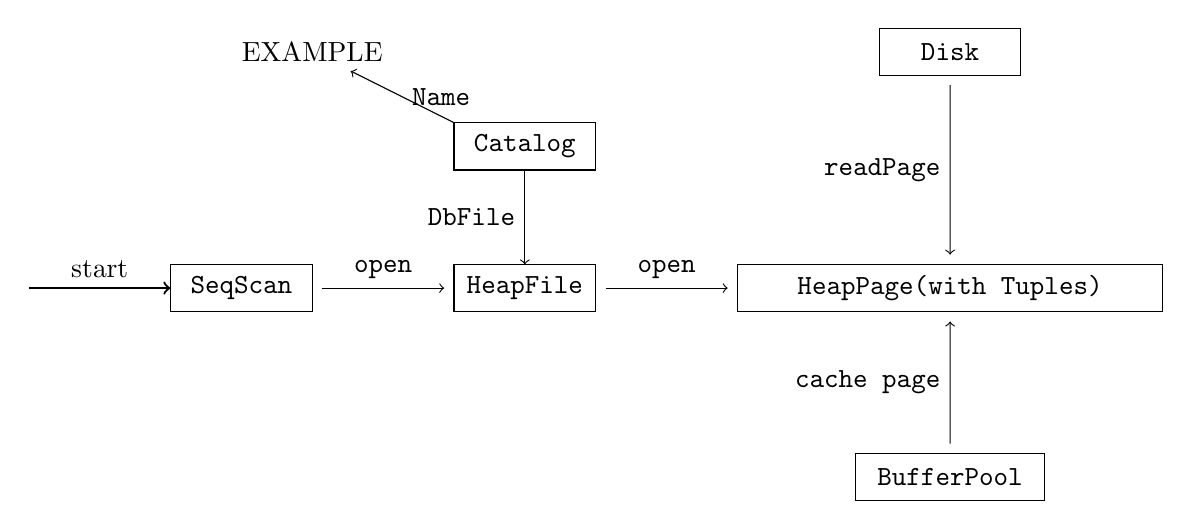
\begin{tikzpicture}[
            scale=.6,
        ]
            \path[->, thick] (-3, -0.5) edge node[midway, above] {start} (0, -0.5);
            \draw[draw=black] (0, 0) rectangle (3, -1) node[midway]  {\texttt{SeqScan}};
            \node (seq) at (3, -0.5) {};
            \draw[draw=black] (6, 0) rectangle (9, -1) node[midway] {\texttt{HeapFile}};
            \node (heapfilel) at (6, -0.5) {};
            \node (heapfiler) at (9, -0.5) {};
            \path[->] (seq) edge node[midway, above] {\texttt{open}} (heapfilel);
            \draw[draw=black] (12, 0) rectangle (21, -1) node[midway] {\texttt{HeapPage(with Tuples)}};
            \node (pagel) at (12, -0.5) {};
            \node (pager) at (21, -0.5) {};
            \node (pageu) at (16.5, 0) {};
            \node (paged) at (16.5, -1) {};
            \path[->] (heapfiler) edge node[midway, above] {\texttt{open}} (pagel);
            \draw[draw=black] (15, 5) rectangle (18, 4) node[midway] {\texttt{Disk}};
            \node (disk) at (16.5, 4) {};
            \path[->] (disk) edge node[midway, left] {\texttt{readPage}} (pageu);
            \draw[draw=black] (14.5, -5) rectangle (18.5, -4) node[midway] {\texttt{BufferPool}};
            \node (buffer) at (16.5, -4) {};
            \path[->] (buffer) edge node[midway, left] {\texttt{cache page}} (paged);
            % catalog
            \draw[draw=black] (6, 3) rectangle (9, 2) node[midway] {\texttt{Catalog}};
            \path[->] (7.5, 2) edge node[midway, left] {\texttt{DbFile}} (7.5, 0);
            \node (name) at (3, 4.5) {EXAMPLE};
            \path[->] (6, 3) edge node[midway, right] {\texttt{Name}} (name);
        \end{tikzpicture}
        \caption{\<SimpleDB> \texttt{open}}
        \label{fig:open}
    \end{figure}

    \begin{figure}[h!]
        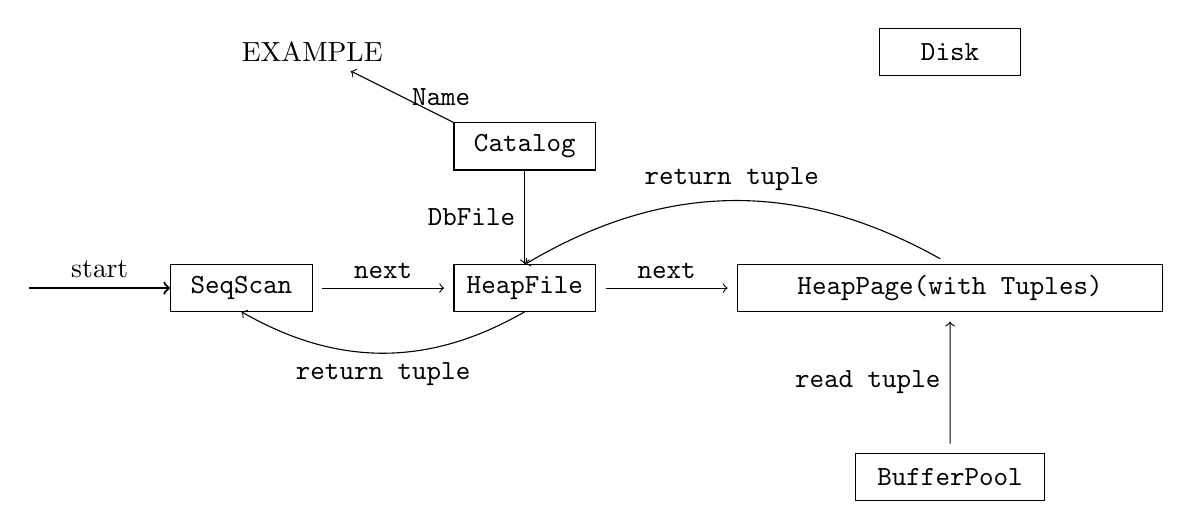
\begin{tikzpicture}[
            scale=.6,
        ]
            \path[->, thick] (-3, -0.5) edge node[midway, above] {start} (0, -0.5);
            \draw[draw=black] (0, 0) rectangle (3, -1) node[midway]  {\texttt{SeqScan}};
            \node (seq) at (3, -0.5) {};
            \draw[draw=black] (6, 0) rectangle (9, -1) node[midway] {\texttt{HeapFile}};
            \node (heapfilel) at (6, -0.5) {};
            \node (heapfiler) at (9, -0.5) {};
            \path[->] (seq) edge node[midway, above] {\texttt{next}} (heapfilel);
            \draw[draw=black] (12, 0) rectangle (21, -1) node[midway] {\texttt{HeapPage(with Tuples)}};
            \node (pagel) at (12, -0.5) {};
            \node (pager) at (21, -0.5) {};
            \node (pageu) at (16.5, 0) {};
            \node (paged) at (16.5, -1) {};
            \path[->] (heapfiler) edge node[midway, above] {\texttt{next}} (pagel);
            \draw[draw=black] (15, 5) rectangle (18, 4) node[midway] {\texttt{Disk}};
            \node (disk) at (16.5, 4) {};
            \draw[draw=black] (14.5, -5) rectangle (18.5, -4) node[midway] {\texttt{BufferPool}};
            \node (buffer) at (16.5, -4) {};
            \path[->] (buffer) edge node[midway, left] {\texttt{read tuple}} (paged);
            \path[->] (pageu) edge [bend right] node[midway, above] {\texttt{return tuple}} (7.5, 0) ;
            \path[->] (7.5, -1) edge [bend left] node[midway, below] {\texttt{return tuple}} (1.5, -1) ;
            \draw[draw=black] (6, 3) rectangle (9, 2) node[midway] {\texttt{Catalog}};
            \path[->] (7.5, 2) edge node[midway, left] {\texttt{DbFile}} (7.5, 0);
            \node (name) at (3, 4.5) {EXAMPLE};
            \path[->] (6, 3) edge node[midway, right] {\texttt{Name}} (name);
        \end{tikzpicture}
        \caption{\texttt{SimpleDB} \texttt{next}}
        \label{fig:next}
    \end{figure}
        In Lab 1, we implemented \<getPage> which is needed for reading pages into memory and getting tuples,
        together with \<SeqScan> operator to scan files and return tuples. The workflow of opening opertators
        to read file and caching pages into BufferPool is shown by Figure \ref{fig:open}, and the workflow of recursively
        getting tuples through \<SeqScan> using \<next()> is shown by Figure \ref{fig:next}. \par

        In Lab 2, we added \<insert>, \<delete> funcionalities in \<SimpleDB>, which insert/delete tuples to/from the
        pages in BufferPool by calling the method from \<HeapFile> to update pages, then \<BufferPool>
        updates the records by re-inserting the pages into the \<BufferPool>. When \<BufferPool> is
        full and a new page need adding, \<writePage> from \<HeapFile> will be called to write a dirty
        page to disk and add the new page into the \<BufferPool>. \<BufferPool> is in charge of updating
        pages because \<Insert/Delete> operators directly call \<insert/delete> of \<BufferPool>. Besides, we also
        implemented \<Filter>, \<Join> operators and the aggregates. As an example, Figure \ref{fig:join} shows the
        workflow of using \<Join> opeator and Figure \ref{fig:insert} shows the workflow of inserting tuples.

        \begin{figure}[htb!]
            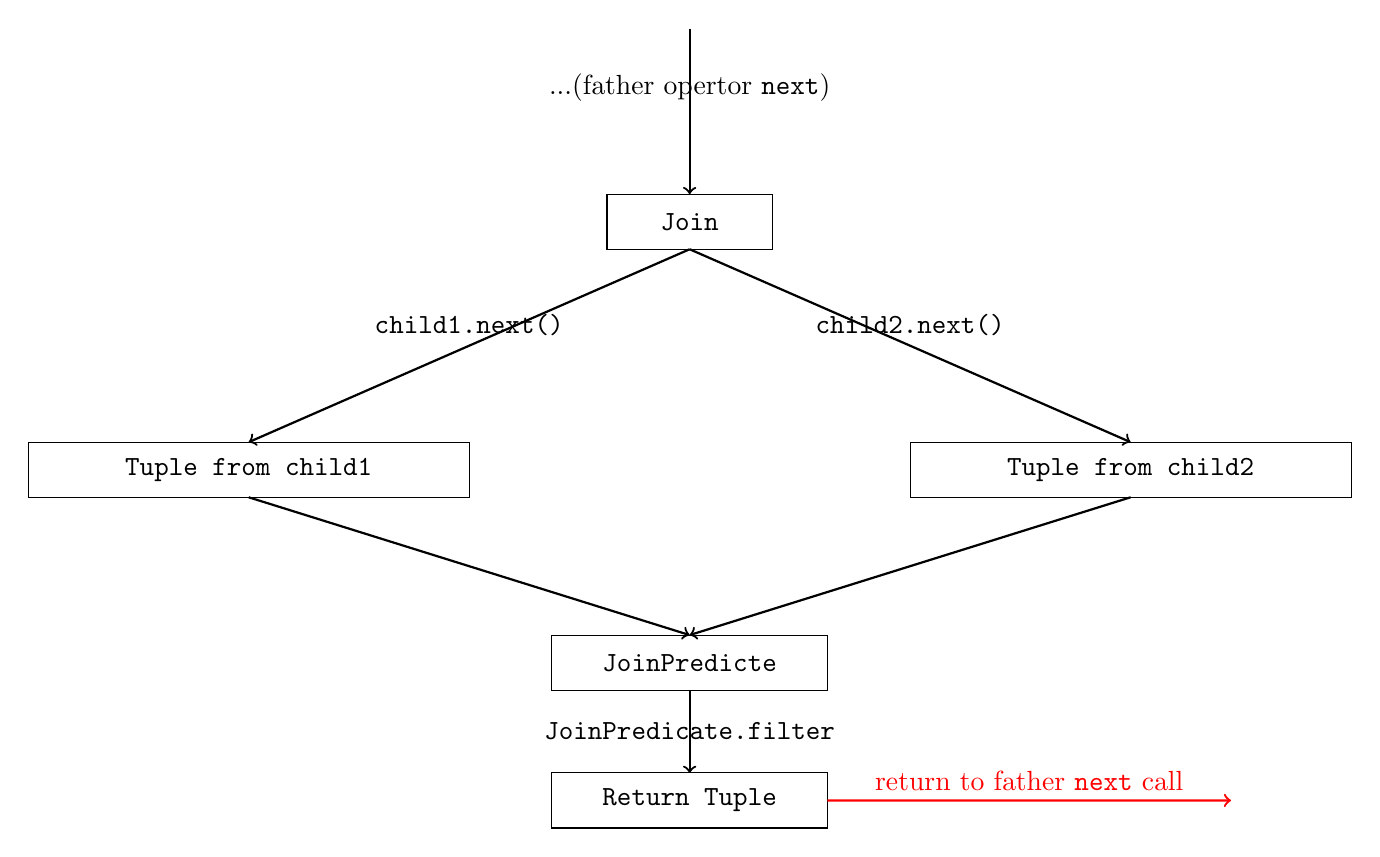
\begin{tikzpicture}[
                scale=.7,
            ]
                \path[->, thick] (0, 3) edge node[midway, above] {...(father opertor \texttt{next})} (0, 0);
                \draw[draw=black] (-1.5, 0) rectangle (1.5, -1) node[midway]  {\texttt{Join}};
                \path[->, thick] (0, -1) edge node[midway, above] {\texttt{child1.next()}} (-8, -4.5);
                \path[->, thick] (0, -1) edge node[midway, above] {\texttt{child2.next()}} (8, -4.5);
                \draw[draw=black] (-12, -4.5) rectangle (-4, -5.5) node[midway]  {\texttt{Tuple from \texttt{child1}}};
                \draw[draw=black] (4, -4.5) rectangle (12, -5.5) node[midway]  {\texttt{Tuple from \texttt{child2}}};
                \path[->, thick] (-8, -5.5) edge node[midway, above] {} (0, -8);
                \path[->, thick] (8, -5.5) edge node[midway, above] {} (0, -8);
                \draw[draw=black] (-2.5, -8) rectangle (2.5, -9) node[midway]  {\texttt{JoinPredicte}};
                \path[->, thick] (0, -9) edge node[midway] {\texttt{JoinPredicate.filter}} (0, -10.5);
                \draw[draw=black] (-2.5, -10.5) rectangle (2.5, -11.5) node[midway]  {\texttt{Return Tuple}};
                \node (father) at (10, -11) {};
                \path[->, thick, color=red] (2.5, -11) edge node[midway, above] {return to father \texttt{next} call} (father);

            \end{tikzpicture}
            \caption{\<SimpleDB join>}
            \label{fig:join}
        \end{figure}

    \subsection{Lock Manager}
    Lab 3 focuses on adding transactions functionality to simpleDB. In order to achieve this, we implemented our own
    \texttt{Lock} and \texttt{LockManager} which together handle acquiring/releasing both \texttt{SHARED} (read-only)
    and \texttt{EXCLUSIVE} (read-write) locks by different transactions on page granularity. \<SimpleDB> uses time-
    out limits for \texttt{acquire} so that a certain period time of blocking on \texttt{acquire} will be considered as
    deadlock and thus cause the system to abort the transaction. \par

    \begin{figure}[htb!]
        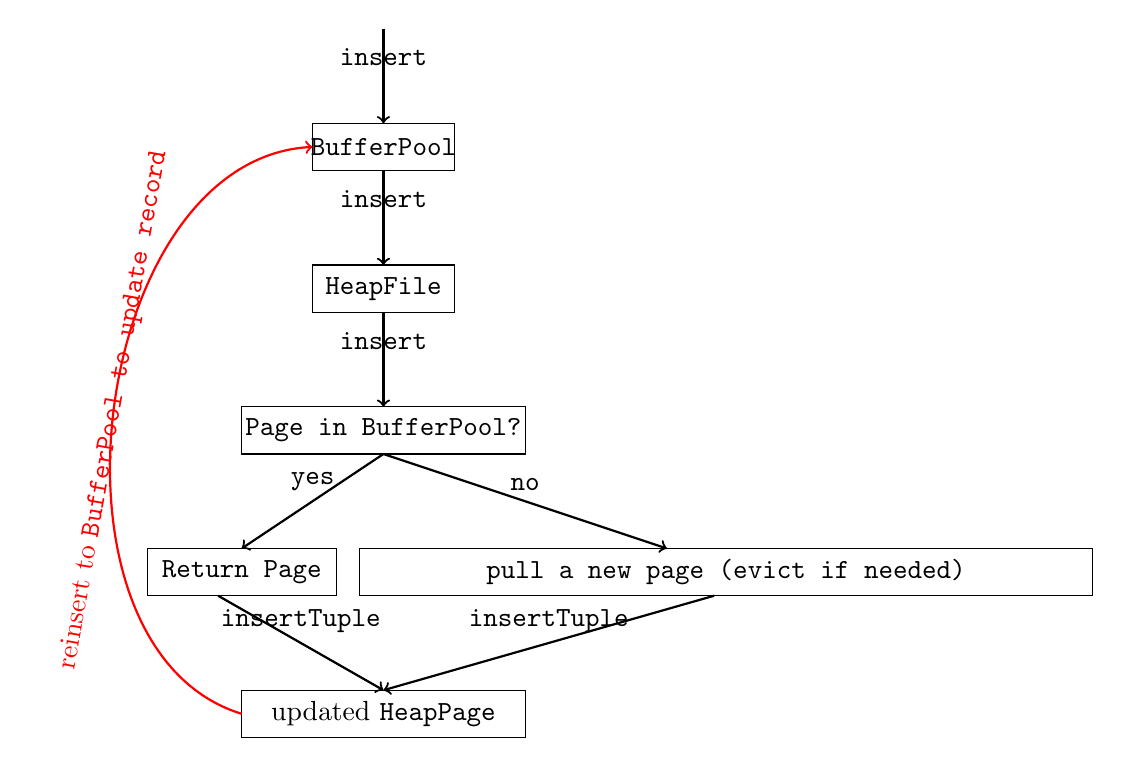
\begin{tikzpicture}[
            scale=.6,
        ]
            \path[->, thick] (0, 2) edge node[midway, above] {\texttt{insert}} (0, 0);
            \draw[draw=black] (-1.5, 0) rectangle (1.5, -1) node[midway]  {\texttt{BufferPool}};
            \path[->, thick] (0, -1) edge node[midway, above] {\texttt{insert}} (0, -3);
            \draw[draw=black] (-1.5, -3) rectangle (1.5, -4) node[midway]  {\texttt{HeapFile}};
            \path[->, thick] (0, -4) edge node[midway, above] {\texttt{insert}} (0, -6);
            \draw[draw=black] (-3, -6) rectangle (3, -7) node[midway]  {\texttt{Page in BufferPool?}};
            \path[->, thick] (0, -7) edge node[midway, above] {\texttt{yes}} (-3, -9);
            \path[->, thick] (0, -7) edge node[midway, above] {\texttt{no}} (6, -9);
            \draw[draw=black] (-5, -9) rectangle (-1, -10) node[midway]  {\texttt{Return Page}};
            \draw[draw=black] (-0.5, -9) rectangle (15, -10) node[midway]  {\texttt{pull a new page (evict if needed)}};
            \path[->, thick] (-3.5, -10) edge node[midway, above] {\texttt{insertTuple}} (0, -12);
            \path[->, thick] (7, -10) edge node[midway, above] {\texttt{insertTuple}} (0, -12);
            \draw[draw=black] (-3, -12) rectangle (3, -13) node[midway]  {updated \texttt{HeapPage}};
            \path[->, thick, color=red] (-3, -12.5) edge [bend left=80] node[midway, rotate=80] {reinsert to \texttt{BufferPool
                to update record}} (-1.5, -0.5);
        \end{tikzpicture}
        \caption{\<SimpleDB insertTuple>}
        \label{fig:insert}
    \end{figure}

	\begin{itemize}
        \item \texttt{Lock}: I need this class to represent the two types of locks simpleDB uses: \texttt{SHARED} and
            \texttt{EXCLUSIVE}. A shared lock is acquired by read-only transactions, and thus can be shared between
            many read-only transactions; an exclusive lock is acquired by read-write transactions, and thus can only be
            acquired by at most one read-write transaction at a time.
        \item \texttt{LockManager}: I need this class as the manager for all locking-related actions in simpleDB. It
            is created within \texttt{BufferPool} and will be called to acquire locks when \texttt{getPage} is called
            and release locks when \texttt{transactionComplete} is called. Note that because of the design of simpleDB,
            \texttt{acquire} in \texttt{LockManager} should only need calling in \texttt{getPage} when simpleDB wants to
            interact with a page. There are a few conditions when \texttt{acquire} will not be a blocking call. They are:
                \begin{itemize}
                    \item When the lock on that page is not locked.
                    \item When the lock is locked by this transaction itself (will upgrade a share lock to
                        exclusive if this transaction is the only one which holds the lock)
                    \item When the lock is locked, but it is a shared lock, and the transaction wants a shared lock.
                \end{itemize}
        \item \texttt{BufferPool.transactionComplete}: I add this method to release all locks acquired by a
            transaction when it commits.
	\end{itemize}

    \subsection{Log Manager}
    In Lab 4, we focus on adding rollback and recovery functionality to \<SimpleDB> upon abort and system crash.
    Specifically, Iweimplemented STEAL (dirty pages may be evicted from the buffer pool even though the transaction
    hasn't commited yet), and NO FORCE (on transaction commit, no need to force write dirty pages to disk) for buffer
    pool management. In order to achieve this, we implemented log-based rollback and recovery which performs a
    redo-phase and an undo-phase. \par

    \<SimpleDB> supports six kinds of logs: \<BEGIN, COMMIT, ABORT, UPDATE, CHECKPOINT,> and \<CLR>. CLR is part of my
    design to make undo-phase easier to implement.

    \begin{itemize}
        \item \texttt{LogFile.rollback}: we need this method to roll back changes made by an aborted transaction. This
        method will read from the end of the log file and undo changes made by this transaction until its first active
        log record. It is also implemented that undo changes will append new CLR logs.

        \item \texttt{LogFile.recover}: I need this method to recover a simpleDB system upon unexpected crashes. It
        will start redoing from the beginning of the log file or the last checkpoint log if any, during which a map of
        active transactions to their first active log line is built. Then, undo-phase will use the active transaction
        map and undo any changes made by these transactions bottom up.
	\end{itemize}

\section{Parallel Data Processing}
	\label{parallel}

    In Lab 6, we added the ability of parallel data processing to \<SimpleDB>. The basic structure of parallel \<SimpleDB>
    contains multiple \<Worker> and one single \<Server>. The workflow goes as follows: for every query the user enters,
    it is first sent to
    \<Server> for some optimization (we did not implement this part this quarter). Next step is to prepare this query to
    be run in parallel by inserting new operators (more on this later). Then this query will be sent to all
    available workers. After each worker receives the query, it will localize it (more on this later) and run the query.
    Finally, each worker will send the results back to \<Server>, then server will aggregate all the results and send
    the final result back to users. \par

    Our implementation of parallel \<SimpleDB> focuses on the following subparts of implementing a functional model:
    \begin{itemize}
        \item How to localize a query to run it on a local machine? (\<Worker.java>)
        \item How to transfer data in between workers? (\<ShuffleProducer.java> \& \<ShuffleConsumer.java>)
        \item How to optimize aggregate performance in a parallel setting? (\<AggreagateOptimizer.java>)
    \end{itemize}
    The following sections explain the detailed implementations on these questions.

    \subsection{\<Worker.java>}
    In \<Worker.java>, we localize the query for it to run on the local machine. It does three jobs: (1) For \<SeqScan>
    operators, reset its \<tid> and \<alias>. This is because the \<tid> of the \emph{local} table may not be the
    same as the one of global table, and the \<Catalog> is a local verlsion. We need to update the \<tid> so that
    \<SeqScan> reads the correct subtable; (2) For \<Producers>, set its worker to \<this>. This is because \<Worker>
    handles the data buffer of \<Consumers> (more on this later) and the \<Producer> needs to know to which bufffer to
    send data for the \<Consumer>; (3) For \<Consumers>, set its data buffer in \<Worker> through its
    \<inBuffer> map.

    \subsection{\<ShuffleProducer.java> \& \<ShuffleConsumer.java>}
    We implement \<ShuffleProducer.java> \& \<ShuffleConsumer.java> to enable data transfer between workers. In
    \<ShuffleProducer.java>, we use the same protocol in \<CollectProducer> to send tuples to \<Consumer>. The difference
    is that \<ShuffleProducer> handles multiple connections with multiple \<ShuffleConsumer> (whose addresses
    are stored in a \<SocketInfo> wrapper), so I keep three lists of \<IoSession> as connections, \<List> as data buffers,
    and \<Long> as timestamps, one combination for one \<Consumer>. The working thread of \<ShuffleProducer> takes
    tuples from its child operator, and uses a \<PartitionFunction> to decide to which consumer to send this tuple. \par

    In \<ShuffleConsumer>, I followed the design of \<CollectConsumer> to constantly take tuples out of the buffer (
    populated by \<ShuffleProducer>) and returns an iterator of tuples in \<fetchNext>. Together, \<ShuffleProducer>
    and \<ShuffleConsumer> enable data transfer between \<Workers>

    \subsection{\<AggregateOptimizer>}
    In \<AggregateOptimizer.java>, we added optimization for aggregates running in parallel. The idea is that each local
    worker could work out an local aggregate result, then sent it to a \<CollectConsumer> to return a final aggregate
    result. For each of the following aggregate, we optimize the performance by:
    \begin{itemize}
        \item \<MIN>: calculate local \<MIN> (downAgg), then take global \<MIN> (upAgg).
        \item \<MAX>: calculate local \<MAX> (downAgg), then take global \<MAX> (upAgg).
        \item \<COUNT>: calculate local \<COUNT> (downAgg), then take global \<SUM> (upAgg).
        \item \<SUM>: calculate local \<SUM> (downAgg), then take global \<SUM> (upAgg).
        \item \<AVG>: locally calculate a \<SUM> and a \<COUNT> (downAgg), then take global
            $\frac{\sum\text{\<SUM>}}{\sum\text{\<COUNT>}}$ (upAgg).
    \end{itemize}

    As an example, Figure \ref{fig:para} is a diagram showing the workflow of Parallel \<SimpleDB> with two workers.
    \begin{figure}[t!]
        \begin{tikzpicture}[
            >=latex,shorten >=2pt,shorten <=2pt,shape aspect=1,
        ]
            \tikzstyle{cyl} = [cylinder, shape border rotate=90, draw, minimum height=1cm, minimum width=5cm]
            \tikzstyle{noo} = [rectangle, draw, minimum height=1pt, minimum width=2pt]
            \tikzstyle{cir} = [ellipse, draw, minimum height=1cm, minimum width=2cm]
            \tikzstyle{poi} = [ellipse, draw, fill]
            \tikzstyle{joining} = []
            \tikzset{>=stealth}
            \tikzstyle{readup} = [red, ->]
            \tikzstyle{comm} = [blue, ->]

            % server
            \node[noo] (user) {User};
            \node[noo, minimum height=1cm, minimum width=3cm, right=1.5cm of user] (server) {Server};
            \node[noo, fill=gray!20, minimum height=0.5cm, minimum width=0.5cm] (cc) at ($(server) + (1.5, 0)$) {CC};
            \path[->] (user) edge node[midway, above] {query} (server);
            \node[rotate=90] (a) at ($(server.south) + (-2, -2)$) {\small{Optimize query}};
            \node[rotate=90] (b) at ($(server.south) + (2, -2)$) {\small{Parallelize query}};
            \path[->] (server.south) edge (a);
            \path[->] (server.south) edge (b);

            % Worker
            \node[noo, minimum height=1cm, minimum width=3cm, above right=1.5cm and 1cm of server]
                (worker11) {Worker 1};
            \node[noo, fill=gray!20, minimum height=0.5cm, minimum width=0.5cm] (sp1) at ($(worker11) + (1.5, 0)$) {SP};
            \path[->] (server.north east) edge node[midway, left] {new query} (worker11);
            \node (c) at ($(worker11.north) + (0, 1)$) {\small{localize query, SeqScan}};
            \path[->] (worker11.north) edge (c);
            \node[noo, minimum height=1cm, minimum width=3cm, right=2cm of worker11] (worker12) {Worker 1};
            \node[noo, fill=gray!20, minimum height=0.5cm, minimum width=0.5cm] (sc1) at ($(worker12) + (-1.5, 0)$) {SC};
            \path[->] (sp1) edge (sc1);

            \node[noo, minimum height=1cm, minimum width=3cm, below right=1.5cm and 1cm of server]
                (worker21) {Worker 2};
            \node[noo, fill=gray!20, minimum height=0.5cm, minimum width=0.5cm] (sp2) at ($(worker21) + (1.5, 0)$) {SP};
            \path[->] (server.south east) edge node[midway, right] {new query} (worker21);
            \node (d) at ($(worker21.south) + (0, -1)$) {\small{localize query, SeqScan}};
            \path[->] (worker21.south) edge (d);
            \node[noo, minimum height=1cm, minimum width=3cm, right=2cm of worker21] (worker22) {Worker 2};
            \node[noo, fill=gray!20, minimum height=0.5cm, minimum width=0.5cm] (sc2) at ($(worker22) + (-1.5, 0)$) {SC};
            \path[->] (sp2) edge (sc2);
            \path[->] (sp1) edge (sc2);
            \path[->] (sp2) edge (sc1);

            \node (e) at ($(worker12) + (0, 2)$) {\small{more processing}};
            \path[->] (worker12.north) edge (e);
            \node (f) at ($(worker22) + (0, -2)$) {\small{more processing}};
            \path[->] (worker22.south) edge (f);
            \node[noo, fill=gray!20, minimum height=0.5cm, minimum width=0.5cm] (cp1) at ($(worker12) + (1.5, 0)$) {CP};
            \node[noo, fill=gray!20, minimum height=0.5cm, minimum width=0.5cm] (cp2) at ($(worker22) + (1.5, 0)$) {CP};
            \path[->, red] (cp1) edge [bend left=15] node[midway, above] {return} (cc);
            \path[->, red] (cp2) edge [bend right=15] node[midway, above] {return} (cc);
            \path[->, red] (cc.west) edge [bend right=30] node[midway, above] {return} (user.north);
        \end{tikzpicture}
        \caption{Parallel \<SimpleDB>. SC - Shuffle Consumer, CC - Collect Consumer, SP - Shuffle Producer, SC - Shuffle
        Consumer}
        \label{fig:para}
    \end{figure}

    \subsection{Performance}
    In this section, I list the performance of parallel \<SimpleDB> running four different queries, with 1, 2, and 4
    workers available. Table \ref{tab:cold} and table \ref{tab:warm} shows the execution time of the following four
    queries on 1, 2, and 4 workers respectively, one for the cold cache (first time running the query since \<SimpleDB>
    starts), the other one for already loaded cache (second time running the query since \<SimpleDB> starts). All runtime
    is the average of six trials.

    Query A:
    \begin{lstlisting}[language=SQL]
    SELECT *
        FROM Actor WHERE id < 1000;
    \end{lstlisting}

    Query B:
    \begin{lstlisting}[language=SQL]
    SELECT m.name,m.year,g.genre
        FROM Movie m, Director d, Genre g, Movie_Director md
        WHERE d.fname='Steven' AND d.lname='Spielberg'
            AND d.id=md.did AND md.mid=m.id
            AND g.mid=m.id;
    \end{lstlisting}

    Query C:
    \begin{lstlisting}[language=SQL]
    SELECT m.name, COUNT(a.id)
        FROM Movie m, Director d, Movie_Director md, Actor a, Casts c
        WHERE d.fname='Steven' AND d.lname='Spielberg'
            AND d.id=md.did AND md.mid=m.id
            AND c.mid=m.id
            AND c.pid=a.id
        GROUP BY m.name;
    \end{lstlisting}

    Query D:
    \begin{lstlisting}[language=SQL]
    SELECT m.name, AVG(a.id)
        FROM Movie m, Director d, Movie_Director md, Actor a, Casts c
        WHERE d.fname='Steven' AND d.lname='Spielberg'
            AND d.id=md.did AND md.mid=m.id
            AND c.mid=m.id
            AND c.pid=a.id
        GROUP BY m.name;
    \end{lstlisting}

    \begin{table}[!htb]
        \centering
        \begin{tabularx}{\linewidth}{Y|Y|Y|Y|Y}
             & \multicolumn{4}{c}{Query} \\ \hline
             \rowcolor{Gray}
             \# workers & A & B & C & D \\\hline
             1 & 1.44 & 1.83 & 5.65 & 5.49 \\\hline
             2 & 1.89 & 1.86 & 5.11 & 6.18 \\\hline
             4 & 1.48 & 3.11 & 7.49 & 7.22 \\
        \end{tabularx}
        \caption{Performance with cold cache}\label{tab:cold}
    \end{table}

    \begin{table}[!htb]
        \centering
        \begin{tabularx}{\linewidth}{Y|Y|Y|Y|Y}
             & \multicolumn{4}{c}{Query} \\ \hline
             \rowcolor{Gray}
             \# workers & A & B & C & D \\\hline
             1 & 1.18 & 0.97 & 4.09 & 4.10 \\\hline
             2 & 1.00 & 1.19 & 3.50 & 3.49 \\\hline
             4 & 1.15 & 1.31 & 4.92 & 4.48 \\
        \end{tabularx}
        \caption{Performance with loaded cache}\label{tab:warm}
    \end{table}

    As shown in the following bar charts (Figure \ref{fig:cold} and Figure \ref{fig:warm}), increasing the number of
    workers seems to \emph{decrease} the performance of \<SimpleDB>. I suspect the reason to be that the size of the
    database we run is not large enough to show the advantage of data processing, i.e. the inner process communication
    time beats the efficiency of parallel execution.

    % prepare data
    \pgfplotstableread[row sep=\\,col sep=&]{
        worker & A & B & C & D\\
        1 & 1.44 & 1.83 & 5.65 & 5.49 \\
        2 & 1.89 & 1.86 & 5.11 & 6.18 \\
        4 & 1.48 & 3.11 & 7.49 & 7.22 \\
    }\colddata

    \pgfplotstableread[row sep=\\,col sep=&]{
        worker & A & B & C & D \\
        1 & 1.18 & 0.97 & 4.09 & 4.10 \\
        2 & 1.00 & 1.19 & 3.50 & 3.49 \\
        4 & 1.15 & 1.31 & 4.92 & 4.48 \\
    }\loaddata

    \begin{figure}[!htb]
        \centering
        \begin{tikzpicture}
            \begin{axis}[
                ybar,
                bar width=.3cm,
                width=.8\textwidth,
                height=.5\textwidth,
                legend style={at={(0.5,1)}, anchor=north,legend columns=-1},
                symbolic x coords={1, 2, 4},
                xtick=data,
                nodes near coords,
                every node near coord/.append style={font=\tiny},
                nodes near coords align={vertical},
                ymin=0,ymax=10,
                ylabel={Execution Time /sec},
                xlabel={\# Workers}
            ]
            \addplot table[x=worker,y=A]{\colddata};
            \addplot table[x=worker,y=B]{\colddata};
            \addplot table[x=worker,y=C]{\colddata};
            \addplot table[x=worker,y=D]{\colddata};
            \legend{A, B, C, D}
        \end{axis}
        \end{tikzpicture}
        \caption{Performance with cold cache}
        \label{fig:cold}
    \end{figure}

    \begin{figure}[!t]
        \centering
        \begin{tikzpicture}
            \begin{axis}[
                ybar,
                bar width=.3cm,
                width=.8\textwidth,
                height=.5\textwidth,
                legend style={at={(0.5,1)}, anchor=north,legend columns=-1},
                symbolic x coords={1, 2, 4},
                xtick=data,
                nodes near coords,
                every node near coord/.append style={font=\tiny},
                nodes near coords align={vertical},
                ymin=0,ymax=10,
                ylabel={Execution Time /sec},
                xlabel={\# Workers}
            ]
            \addplot table[x=worker,y=A]{\loaddata};
            \addplot table[x=worker,y=B]{\loaddata};
            \addplot table[x=worker,y=C]{\loaddata};
            \addplot table[x=worker,y=D]{\loaddata};
            \legend{A, B, C, D}
        \end{axis}
        \end{tikzpicture}
        \caption{Performance with loaded cache}
        \label{fig:warm}
    \end{figure}

\section{Discussion}
	\label{discussion}

    \<SimpleDB> consists most of the modern database architecture \cite{lecture3}. However, there are a
    few aspects in my \<SimpleDB> implementation (for simplicity) which affects the performance. Here are a few:
    \begin{itemize}
        \item Naive \<BufferPool> eviction policy: in the current design, we choose the first page in \<BufferPool> when
            its full. This is a naive approach because the page might be a frequently accessed page. A better approach
            is to use an approximation of Least-Recently-Used policy to evict dirty pages.
        \item Lack of indices: There are no index files in \<SimpleDB> architecture, which is a drastic decrease performance
            wise, especially for databases which receive more look-up queries.
        \item Slow join: The current implementation of join is nested-loop-join, which is the least efficient. Ideally,
            to achieve the fastest join performance, hash-join should be used on equally join and merge-sort-join should
            be used on inequality join.
        \item Slow(and potentially inaccurate) deadlock detection: my current design for deadlock detection is using
            time-out, which bascially terminates a transacation if it has not been successful on grabbing a lock for a
            certain period of time. First, time-out is slow: if a deadlock occurs, the system will have to wait until the
            time-out limit is reached. Second, time-out may be inaccurate: imagine a course registration database -- there
            are centainly times when a great number of transactions want to access the same resource, so natually the
            wait time for a single transaction would be longer. Time-out might terminate a transaction which is not deadlocked --
            it might just be slow. This is worse when the transaction has done a lot of work before this lock. Then whole
            work will be need to be redone. Therefore, a dependency graph would be a better choice, for many transactions
        \item Page-granularity lock: The lock is per-\<HeapPage> for the current design. A tuple-granularity lock would
            bring faster performance, but more complex synchronization issue and memory need.
        \item Recovery Protocal: we did not implement ARIES \cite{lecture18}, as discussed in class.
            Instead, current design of redoing every log is wasteful.
    \end{itemize}

\newpage
\begin{thebibliography}{9}
    \bibitem{lecture3}
    Balazinska, Mass, Lecture 3
    \\\texttt{https://courses.cs.washington.edu/courses/cse444/18wi/lectures/lecture03-architecture-large.pdf}
    \bibitem{lecture18}
    Balazinska, Mass, Lecture 18
    \\\texttt{https://courses.cs.washington.edu/courses/cse444/18wi/lectures/lecture17-19-transactions-recovery-large.pdf}
    \bibitem{db}
    SimpleDB Lab ReadME
    \\\texttt{https://gitlab.cs.washington.edu/cse444-18wi/simple-db}


\end{thebibliography}

\end{document}
